%!TEX root = artem_kotov_v1.tex
\section{Task 3}

\begin{task}
    Пронаблюдать, как происходит уточнение прогноза для величины c по мере прихода новой косвенной информации.
\end{task}


\begin{solution}
    \begin{figure}[H]
        \centering
        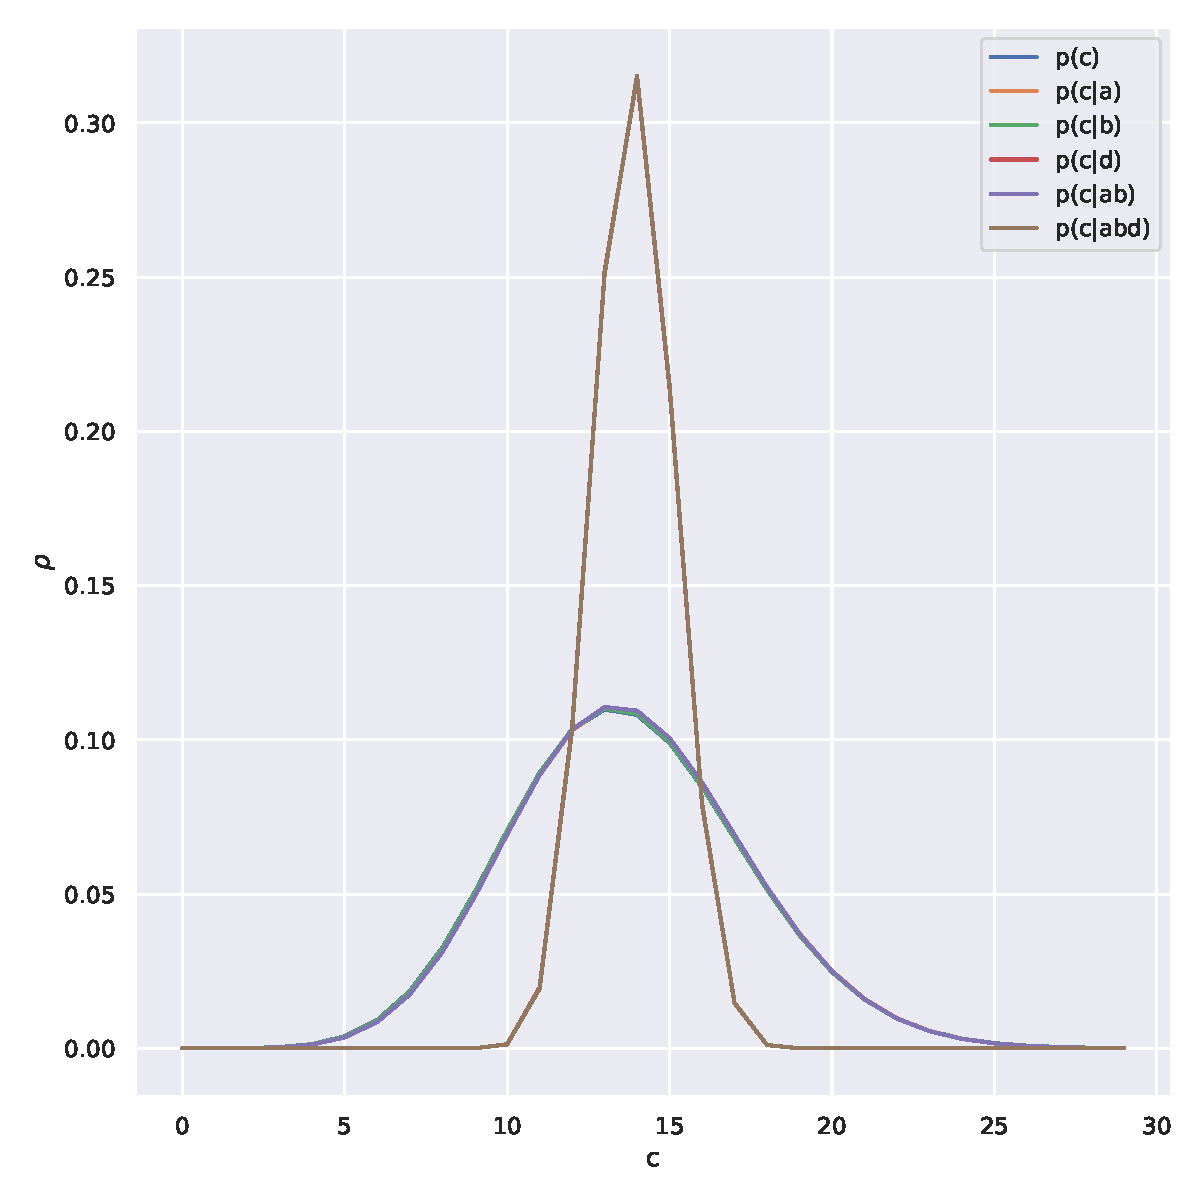
\includegraphics[width=0.7\textwidth]{pics/task3_1.pdf}
        \caption{График плотности распределений $p(c), p(c|a), p(c|b), p(c|d), p(c|ab), p(c|abd)$ для первой модели, где $c \in [0, 30]$, $a, b, d$ равны своим математическим ожиданиям.}
    \end{figure}

    \begin{figure}[H]
        \centering
        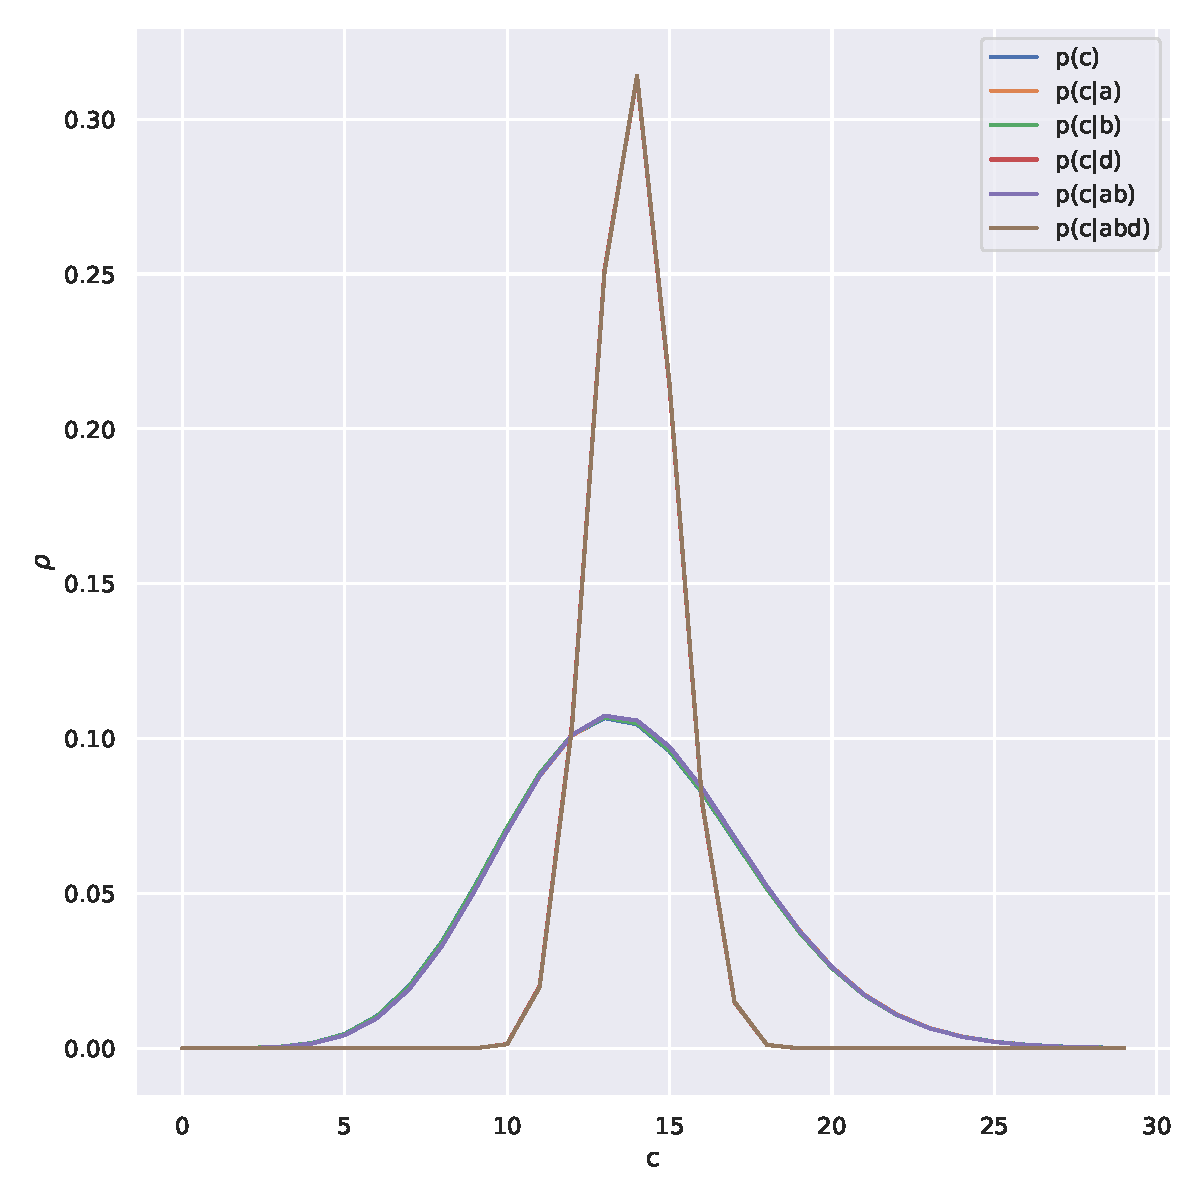
\includegraphics[width=0.7\textwidth]{pics/task3_2.pdf}
        \caption{График плотности распределений $p(c), p(c|a), p(c|b), p(c|d), p(c|ab), p(c|abd)$ для второй модели, где $c \in [0, 30]$, $a, b, d$ равны своим математическим ожиданиям.}
    \end{figure}

    На графиках видно, что многие распределения совпали, так, например, $p(c|d)$ и $p(c|abd)$ крайне похожи для обоих моделей. Также видно, что знание о $d$ существенно уменьшает дисперсию величины $c$, при это дополнительная информация о $a, b$ уже существенно не влияет на распределение.

    \begin{table}[H]
        \centering
        \caption{Мат. ожидания и дисперсии $p(c), p(c|a), p(c|b), p(c|d), p(c|ab), p(c|abd)$, округленные до 2-ух знаков после запятой.}
        \pgfplotstableset{%
            numeric type,
            precision = 2,
            zerofill,
            columns/model/.style={column name={№ Модели}, string type, column type=l},
            columns/type/.style={column name={}, string type, column type=l},
            columns/pc/.style={column name={$p(c)$}, column type=X},
            columns/pc_a/.style={column name={$p(c|a)$}, column type=X},
            columns/pc_b/.style={column name={$p(c|b)$}, column type=X},
            columns/pc_d/.style={column name={$p(c|d)$}, column type=X},
            columns/pc_ab/.style={column name={$p(c|ab)$}, column type=X},
            columns/pc_abd/.style={column name={$p(c|abd)$}, column type=X},
        }
        \pgfplotstabletypeset{./tables/3.csv}
    \end{table}

    Для этих распределений, в целом, аналогично, мат ожидания не чувствуют разницу в моделях, а дисперсии у второй модели систематически больше.
\end{solution}
